\documentclass[10pt]{article}

\usepackage{neurips_msdm5054}
\usepackage[utf8]{inputenc}
\usepackage[T1]{fontenc}
\usepackage{booktabs}
\usepackage{graphicx}
\usepackage{amsmath}
\usepackage{enumitem}
\usepackage{xcolor}
\usepackage[colorlinks=true,linkcolor=blue!60!black,citecolor=blue!60!black,urlcolor=blue!60!black]{hyperref}

\definecolor{todobg}{RGB}{245,247,252}
\definecolor{todoborder}{RGB}{90,115,175}
\newcommand{\teammatebox}[2]{%
  \vspace{4pt}\noindent
  \fcolorbox{todoborder}{todobg}{%
    \parbox{\dimexpr\linewidth-2\fboxsep-2\fboxrule\relax}{%
      \small\textbf{[Pending Module Slot --- #1]}\\[2pt]
      #2%
    }%
  }\vspace{4pt}%
}

\title{Deconstructing Visual Alpha: An Empirical Audit of Inductive Bias, Label Noise, Calibration, and Concept Drift in Financial Chart CNNs}

\author{
  \textbf{Hanchong Qiu} \quad
  \textbf{[Member B Name]} \quad
  \textbf{Dongqing Zhao} \quad
  \textbf{[Member D Name]} \\[3pt]
  Department of Mathematics / Data-Driven Modeling, HKUST \\
  \texttt{hqiu@connect.ust.hk}
}

\begin{document}
\maketitle

% =============================================================================
% ABSTRACT (Drafted with completed Baseline + RQ3 numbers; 1 sentence open for RQ1/2/4)
% =============================================================================
\begin{abstract}
Jiang, Kelly, and Xiu (2023) demonstrate that convolutional neural networks (CNNs) trained directly on binary stock price-and-volume chart images generate economically substantial out-of-sample return forecasts (``Visual Alpha''). Yet from a statistical machine learning perspective, why high-capacity vision architectures succeed in an environment characterized by extreme aleatoric noise ($\text{accuracy} \approx 52\%$) and structural non-stationarity remains insufficiently understood. Using a panel of $2,196,994$ monthly U.S.\ equity chart observations from 1993 to 2019, we build a unified benchmark split by chart date and conduct a four-stage diagnostic audit across the machine learning pipeline: (1) architectural inductive bias and spatial component masking, (2) supervision noise under near-zero return margins and prediction horizons, (3) probability calibration and selective tail prediction, and (4) temporal concept drift and Grad-CAM visual attribution. Our baseline replication confirms that a $708\text{K}$-parameter 2D-CNN trained strictly on 1993--1999 charts achieves a persistent 2000--2019 out-of-sample equal-weighted long-short decile Sharpe ratio of $1.74 \pm 0.19$ across five seeds ($1.68$ for the 5-seed ensemble, $+22.33\%$ annualized spread, $t = 7.51$). Further, deep ensembling cuts expected calibration error by $51.2\%$ ($0.0215 \to 0.0105$) and elevates directional accuracy monotonically from $52.50\%$ at full market coverage to $57.40\%$ in the top-$5\%$ confidence tail, explaining how modest full-sample classification edges translate into strong cross-sectional portfolio performance. Excluding training returns below 5\% in magnitude reduced test AUC from 0.5322 to 0.5170, while retaining all charts and smoothing labels reduced calibration error from 0.0166 to 0.0137. \textit{[Add RQ1 and RQ4 findings at integration.]}
\end{abstract}

% =============================================================================
% SECTION 1: INTRODUCTION & SCIENTIFIC QUESTIONS (Member A — COMPLETE)
% =============================================================================
\section{Introduction and Scientific Questions}

Empirical asset pricing is fundamentally a learning problem under an ultra-low signal-to-noise ratio (SNR). Classical return predictors---such as short-term reversal, intermediate-horizon momentum, and moving-average crossover rules---rely on hand-crafted parametric functionals of lagged returns and trading volume \cite{jegadeesh1993returns,lo2000foundations}. In a landmark study, Jiang, Kelly, and Xiu \cite{jiang2023reimagining} depart from tabular feature engineering by rendering 20-day open-high-low-close (OHLC) bars, moving averages (MA), and volume bars into $64 \times 60$ binary images and training convolutional neural networks (CNNs) to classify the sign of subsequent stock returns. Remarkably, models estimated solely on 1993--1999 charts deliver highly significant long-short portfolio returns over the subsequent two decades without re-estimation.

While economically striking, treating financial chart CNNs as end-to-end black boxes leaves open foundational \emph{statistical machine learning} questions. Unlike natural object recognition---where labels are deterministic, class margins are wide, and visual semantics are time-invariant---financial return classification operates near the Bayes error bound ($P(y=1 \mid x) \in [0.40, 0.60]$), suffers from severe boundary label noise around zero return, and faces institutional regime shifts from fractional floor trading in the 1990s to algorithmic decimalized markets in the 2010s. Simply chasing higher accuracy via ad-hoc architectural tweaks obscures the statistical mechanisms governing generalization.

In this study, we reframe the replication of Jiang et al.\ \cite{jiang2023reimagining} as a systematic \textbf{four-stage statistical ML audit} along the modeling lifecycle. Holding fixed a unified memory-mapped data pipeline and a four-metric evaluation contract over $1.49$ million out-of-sample (OOS) stock-month observations (2000--2019), we formulate four testable scientific questions:
\begin{itemize}[leftmargin=1.6em,itemsep=1.5pt,topsep=2pt]
  \item \textbf{RQ1 (Inductive Bias \& Visual Component Masking):} Does predictive power genuinely require 2D local spatial convolutions, or can flattened linear projections (PCA + Logistic Regression), regional pixel-summary gradient boosting (LightGBM), 1D temporal convolutions, or higher-capacity ResNets match the asymmetric $(5 \times 3)$ CNN? Which visual sub-regions (volume vs.\ price; early vs.\ recent trading days) carry the incremental signal?
  \item \textbf{RQ2 (Supervision Noise, Margin Filtering \& Horizon):} Because binary labels assign opposite classes to $+0.01\%$ and $-0.01\%$ returns, does excluding ambiguous near-zero training observations ($|\text{Retx}_{20d}| < \tau$ or volatility-scaled $|t\text{-stat}| < \tau_t$) or applying label smoothing improve OOS generalization, or does sample reduction induce an adverse bias--variance trade-off? How rapidly does visual predictability decay across 5-, 20-, and 60-day horizons?
  \item \textbf{RQ3 (Probability Calibration \& Selective Prediction):} Are raw CNN return probabilities overconfident? How effectively do post-hoc temperature scaling \cite{guo2017calibration} and multi-seed deep ensembling \cite{lakshminarayanan2017simple} calibrate predicted probabilities, and how does directional accuracy scale when abstaining on uncertain stocks (selective prediction)?
  \item \textbf{RQ4 (Temporal Concept Drift \& Visual Attribution):} Have visual price patterns learned from 1993--1999 degraded in modern algorithmic markets (2013--2019), and can retraining on recent regimes (2006--2012) mitigate concept drift? What economic patterns do individual and population-averaged Grad-CAM \cite{selvaraju2017gradcam} attribution maps reveal?
\end{itemize}

% =============================================================================
% SECTION 2: DATASET, ARCHITECTURE & PROTOCOL (Member A — COMPLETE)
% =============================================================================
\section{Dataset, Baseline Architecture, and Evaluation Protocol}

\subsection{Visual Chart Anatomy, Label Alignment, and Strict Temporal Split}
We study the U.S.\ equity 20-day monthly panel (\texttt{monthly\_20d}) spanning 27 years from 1993 to 2019 ($2,196,994$ raw stock-month observations). At each month-end rebalancing date $t$, the trailing $d \in \{0, \dots, 19\}$ trading days of stock $i$ are rasterized into a single-channel $64 \times 60$ binary matrix $X_{i,t} \in \{0, 255\}^{64 \times 60}$, rescaled on-device to $[0, 1]$. Each trading day occupies exactly three horizontal columns: column $3d$ marks the opening price tick, column $3d+1$ spans the daily high-to-low vertical range and bottom volume bar, and column $3d+2$ marks the closing price tick, overlaid with a continuous 20-day moving-average curve. Vertically, rows \texttt{0:51} ($51\text{ px}$) encode min-max normalized prices within the 20-day window, row \texttt{51} ($1\text{ px}$) is an all-zero separator line verified across all samples, and rows \texttt{52:64} ($12\text{ px}$) encode daily trading volume bars rising from row \texttt{63}. To prevent $34\text{ GB}$ \texttt{float32} memory expansion, raw \texttt{uint8} binary files ($8.6\text{ GB}$) are accessed strictly via read-only \texttt{np.memmap} slices with coalesced per-year batch reads.

\textbf{Supervision vs.\ Portfolio Return Alignment.} A critical empirical subtlety uncovered during schema verification is the distinction between ex-dividend return $\text{Retx}_{20d}$ and dividend-inclusive total return $\text{Ret}_{20d}$. In the benchmark metadata, the official binary target $\text{Retx\_20d\_label} \in \{0, 1, 2\}$ is defined deterministically on \emph{ex-dividend} return: $y_{i,t} = \mathbb{I}(\text{Retx}_{20d,i,t} > 0)$, with code $2$ indicating missing forward returns (whereas $\text{Ret}_{20d}$ differs in sign on $\approx 900$ dividend-paying observations per year). Accordingly, we enforce three invariants across all workstreams: (i) drop missing labels ($y_{i,t} = 2$) first, leaving $2,181,781$ valid observations; (ii) pair any training margin filter strictly with $\text{Retx}_{20d}$ so supervision signs never conflict; and (iii) evaluate realistic investable portfolio returns using total return $\text{Ret}_{20d}$ (falling back to $\text{Retx}_{20d}$ on $0.08\%$ missing entries).

\textbf{Temporal Partition.} Following Jiang et al.\ \cite{jiang2023reimagining}, all primary models are estimated strictly within \textbf{1993--1999} ($689,894$ valid observations), partitioned deterministically (\texttt{seed=42}) into a $70\%$ training set ($N_{\text{train}} = 482,926$) and a $30\%$ validation set ($N_{\text{val}} = 206,968$). The entire 20-year span \textbf{2000--2019} ($N_{\text{test}} = 1,491,887$ valid observations across $240$ monthly cross-sections) is held out untouched for OOS evaluation.

\begin{table}[t]
  \centering
  \caption{\textbf{Baseline 20-Day CNN Out-of-Sample Replication (2000--2019, $N = 1,491,887$).} Models are trained strictly on 1993--1999 ($70/30$ train/val split) with validation cross-entropy early stopping. Portfolio columns report annualized equal-weighted decile long ($D_{10}$), short ($D_1$), and long-short ($D_{10}-D_1$) metrics.}
  \label{tab:baseline}
  \vspace{2pt}
  \resizebox{\textwidth}{!}{%
  \begin{tabular}{lcccccccc}
    \toprule
    \textbf{Model Specification} & \textbf{Acc (\%)} & \textbf{CE Loss} & \textbf{AUC} & \textbf{ECE} & \textbf{Long (\%)} & \textbf{Short (\%)} & \textbf{L--S (\%)} & \textbf{Sharpe ($t$-stat)} \\
    \midrule
    CNN20D (\texttt{seed=42}) & 52.33 & 0.6924 & 0.5322 & 0.0166 & 17.60 & $-3.71$ & 21.32 & 1.70 (7.59) \\
    CNN20D (\texttt{seed=43}) & 52.40 & 0.6926 & 0.5337 & 0.0200 & 19.17 & $-4.48$ & 23.64 & 1.98 (8.86) \\
    CNN20D (\texttt{seed=44}) & 52.15 & 0.6930 & 0.5318 & 0.0203 & 15.96 & $-3.44$ & 19.40 & 1.75 (7.81) \\
    CNN20D (\texttt{seed=45}) & 51.91 & 0.6939 & 0.5255 & 0.0239 & 16.00 & $-0.38$ & 16.39 & 1.47 (6.56) \\
    CNN20D (\texttt{seed=46}) & 51.67 & 0.6945 & 0.5275 & 0.0269 & 16.49 & $-1.08$ & 17.57 & 1.80 (8.07) \\
    \midrule
    Single CNN ($\mu \pm \sigma$, 5 seeds) & $52.09 \pm 0.30$ & $0.6933 \pm 0.0009$ & $0.5301 \pm 0.0035$ & $0.0215 \pm 0.0040$ & $17.04$ & $-2.62$ & $19.66 \pm 2.91$ & $1.74 \pm 0.19$ (7.78) \\
    \textbf{5-Seed Deep Ensemble} & \textbf{52.50} & \textbf{0.6915} & \textbf{0.5355} & \textbf{0.0105} & \textbf{18.19} & $\mathbf{-4.14}$ & \textbf{22.33} & \textbf{1.68 (7.51)} \\
    \bottomrule
  \end{tabular}%
  }
  \vspace{-4pt}
\end{table}

\subsection{Baseline CNN Specification, Unified Metrics, and Replication Benchmark}
We implement the exact 20-day architecture (\texttt{CNN20D}, $708,866$ trainable parameters) illustrated in Jiang et al.\ \cite{jiang2023reimagining}: three convolutional blocks with asymmetric $(5 \times 3)$ filters expanding channels $1 \to 64 \to 128 \to 256$, each followed by 2D batch normalization, LeakyReLU ($\alpha = 0.01$), and vertical $(2 \times 1)$ max-pooling. Following the original design, Block 1 applies vertical stride $(3, 1)$, vertical dilation $(2, 1)$, and padding $(12, 1)$ to capture wide price-range context while preserving all 60 horizontal time columns, yielding a flattened $(256 \times 3 \times 60) = 46,080$-dimensional representation passed through $50\%$ dropout into a 2-way linear head. Weights are initialized via Xavier uniform initialization and optimized using Adam ($\text{lr} = 10^{-5}$, batch size $256$, maximum $15$ epochs) with early stopping (\texttt{patience=2}) on validation cross-entropy loss.

Every model across Sections 2--6 is evaluated via four complementary metrics: (1) \textbf{OOS Directional Accuracy (\%)} at threshold $0.50$; (2) \textbf{Cross-Entropy (CE) Loss} and \textbf{ROC-AUC}; (3) 10-bin confidence \textbf{Expected Calibration Error (ECE)}, $\sum_{m=1}^{10} \frac{|B_m|}{N} |\text{acc}(B_m) - \text{conf}(B_m)|$; and (4) \textbf{Annualized Equal-Weighted Long-Short Decile Sharpe Ratio}, constructed at each month $t$ by ranking stocks on $\hat{p}_{i,t} = P(y_{i,t}=1 \mid X_{i,t})$ into 10 equal-sized deciles and computing $\text{SR}_{\text{ann}} = \sqrt{12}\,\hat{\mu}(R_{D_{10},t} - R_{D_1,t}) / \hat{\sigma}(R_{D_{10},t} - R_{D_1,t})$.

\textbf{Baseline Replication Results.} Table~\ref{tab:baseline} confirms a clean, high-significance replication of Visual Alpha. Individual seeds converge within $5$--$13$ epochs and achieve $52.09\% \pm 0.30\%$ OOS accuracy, $0.5301 \pm 0.0035$ AUC, and an annualized equal-weighted long-short Sharpe ratio of $1.74 \pm 0.19$ ($t$-statistics between $6.56$ and $8.86$, far exceeding the $t > 3.0$ asset-pricing hurdle \cite{gu2020empirical}). Averaging predicted probabilities across all five seeds (\textbf{5-Seed Deep Ensemble}) improves OOS accuracy to $52.50\%$, reduces CE loss to $0.6915$, raises AUC to $0.5355$, and widens the annualized long-short return spread from $19.66\%$ to $22.33\%$ (long leg $+18.19\%$ vs.\ short leg $-4.14\%$, Sharpe $1.68$, $t = 7.51$).

% =============================================================================
% SECTION 3: RQ1 SLOT (Member B)
% =============================================================================
\section{RQ1: Architectural Inductive Bias and Visual Component Ablation}
\teammatebox{Member B --- Section 3 ($\approx 1.4$ pages, includes Table 2 + Figure 1)}{%
  \textbf{Planned Content:} Controlled comparison across five model families trained on identical 1993--1999 splits and evaluated on the full $N=1,491,887$ OOS panel: (B1) Incremental PCA + L2 Logistic Regression, (B2) 48 regional pixel-summary features + LightGBM, (B3) temporal-only 1D-CNN on $(192 \times 20)$ reshaped slices, (B0) Baseline 2D-CNN, and (B4) higher-capacity 1-channel ResNet. Second, occlusion and retraining ablations zeroing out volume bars (\texttt{rows 52:64}), early 10 days (\texttt{cols 0:30}), and recent 10 days (\texttt{cols 30:60}) via \texttt{visual\_alpha.apply\_image\_mask}.%
}

% =============================================================================
% SECTION 4: RQ2 (Member C)
% =============================================================================
\section{RQ2: Does filtering near-zero returns improve supervision?}
\label{sec:sq2}
A return just above zero receives the opposite label to one just below it. We tested whether removing these cases during training improves prediction on future charts. We reused the seed-42 baseline (C0) and trained the same CNN on progressively larger absolute 20-day ex-dividend returns (C1--C3). C4 used the supplied volatility-standardized return with $|t|\geq 0.5$. C5 retained all training charts and assigned probability 0.95 to the observed class. Validation used hard-label cross-entropy (CE) throughout. All six models faced the same 1,491,887 test charts.

\ifnum\value{figure}=0\setcounter{figure}{1}\fi % Figure 1 belongs to pending RQ1.
\begin{figure}[htb]
  \centering
  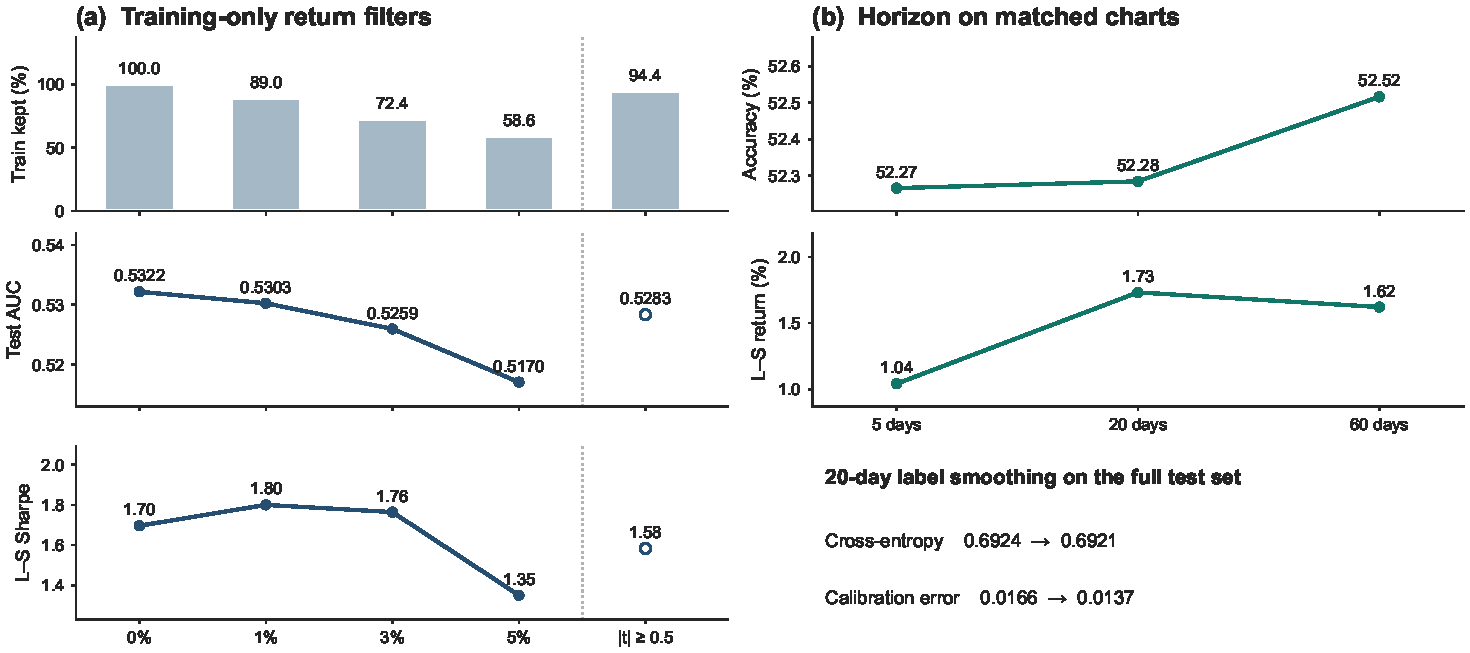
\includegraphics[width=\linewidth]{../outputs/figures/fig2_sq2_noise_horizon.pdf}
  \caption{\textbf{Training filters and forecast horizons, 2000--2019.} (a) Absolute return thresholds and a separate volatility-standardized filter. Retention is relative to 482,926 training charts. (b) Accuracy and mean top-minus-bottom decile holding-period return on 1,471,746 charts with valid targets at all three horizons. The smoothing comparison uses the full 20-day test set.}
  \label{fig:sq2}
\end{figure}

\textbf{Filtering weakened ranking.} As the threshold rose from 0 to 1, 3 and 5\%, test AUC fell at every step (Figure~\ref{fig:sq2}a). At 5\%, the model retained 58.6\% of training charts. Accuracy fell from 52.33\% to 51.34\%, CE rose from 0.6924 to 0.7131, and calibration error (ECE) rose from 0.0166 to 0.0786. The standardized filter retained 94.4\% and gave an AUC of 0.5283. The 5\% filter kept 70.9\% of the smallest and 53.0\% of the largest capitalization quintile among 445,641 training charts with positive recorded capitalization. The source also contains 37,285 negative values, excluded only from this size diagnostic. Changes in sample size and stock mix limit causal interpretation.

\textbf{Average spread and Sharpe gave different answers.} At the 3\% threshold, AUC fell by 0.0062 and Sharpe rose by 0.07. Yet the mean monthly long--short spread fell by 0.373 percentage points (pp). Its paired 95\% interval was $[-0.603,-0.179]$ pp, using 2,000 moving-block resamples of three consecutive months from the 240 paired monthly spreads. With label smoothing, CE fell by 0.00030 and ECE by 0.00286. The mean spread changed by $+0.023$ pp (95\% interval $[-0.108,+0.164]$ pp). These intervals describe variation across months for the fitted models. Each variant was trained once, and the reused baseline need not share its initial weights.

\textbf{The strongest horizon depended on the metric.} On matched charts, 60 days gave the highest accuracy (52.52\%) and the highest up-label frequency (51.51\%). At 5, 20 and 60 days, AUC was 0.5298, 0.5315 and 0.5296, respectively. The 20-day model also had the largest mean holding-period spread (1.73\%, versus 1.04\% and 1.62\%). Signals occur once a month and 60-day holdings overlap. Returns therefore cover different lengths of time. Splitting by chart date also allows late-1999 forward labels to extend into 2000.

% =============================================================================
% SECTION 5: RQ3 CALIBRATION & SELECTIVE PREDICTION (Member A — COMPLETE)
% =============================================================================
\section{RQ3: Probability Calibration, Deep Ensembling, and Selective Prediction}

\subsection{Statistical Motivation and Calibration Methodology}
In portfolio construction and risk-sensitive decision making, a classifier's predicted probability $\hat{p}_{i,t} = P(y_{i,t}=1 \mid X_{i,t})$ is consumed not merely as an ordinal score, but as a cardinal estimate of expected directional edge $|\hat{p}_{i,t} - 0.5|$. Modern neural networks trained with unregularized cross-entropy frequently exhibit probability overconfidence \cite{guo2017calibration}, an issue compounded in financial panels where irreducible market shocks bound true conditional probabilities close to $0.50$.

We investigate two principled calibration mechanisms requiring \emph{zero} architectural changes:
\begin{enumerate}[leftmargin=1.6em,itemsep=1.5pt,topsep=2pt]
  \item \textbf{Post-Hoc Temperature Scaling \cite{guo2017calibration}:} Given validation logits $(z_{0}, z_{1})$, we fit a single scalar temperature $T > 0$ via L-BFGS to minimize negative log-likelihood strictly on the 1993--1999 validation split ($N_{\text{val}} = 206,968$), producing calibrated OOS probabilities $\hat{p}^{(T)} = \sigma((z_1 - z_0)/T)$. Because $z \mapsto z/T$ is strictly monotonic for $T > 0$, temperature scaling isolates pure probability calibration while leaving rank-based metrics (AUC and decile Sharpe) invariant.
  \item \textbf{Multi-Seed Deep Ensembling \cite{lakshminarayanan2017simple}:} We average predictive probabilities $\bar{p}_{i,t} = \frac{1}{K}\sum_{k=1}^K \hat{p}^{(k)}_{i,t}$ across $K = 5$ independently initialized \texttt{CNN20D} models (\texttt{seeds} $42\text{--}46$), reducing epistemic estimation variance induced by non-convex optimization and $50\%$ dropout.
\end{enumerate}

\begin{table}[t]
  \centering
  \caption{\textbf{RQ3 Calibration Summary on 2000--2019 OOS Test Set ($N = 1,491,887$).} Scalar temperatures $T$ are estimated strictly on the 1993--1999 validation split without touching OOS data.}
  \label{tab:sq3}
  \vspace{2pt}
  \resizebox{\textwidth}{!}{%
  \begin{tabular}{lccccccc}
    \toprule
    \textbf{Calibration Method} & \textbf{Fitted $T$} & \textbf{Acc (\%)} & \textbf{CE Loss} & \textbf{AUC} & \textbf{ECE $\downarrow$} & \textbf{L--S (\%)} & \textbf{Sharpe} \\
    \midrule
    Single CNN (\texttt{seed=42}, Uncalibrated) & $1.000$ & 52.33 & 0.6924 & 0.5322 & 0.0166 & 21.32 & \textbf{1.70} \\
    Single CNN + Temp Scaling & $1.064$ & 52.33 & 0.6921 & 0.5322 & 0.0142 & 21.32 & \textbf{1.70} \\
    \textbf{5-Seed Deep Ensemble} & $1.000$ & \textbf{52.50} & \textbf{0.6915} & \textbf{0.5355} & \textbf{0.0105} & 22.33 & 1.68 \\
    5-Seed Ensemble + Temp Scaling & $0.878$ & 52.50 & 0.6920 & 0.5355 & 0.0155 & \textbf{22.35} & 1.68 \\
    \bottomrule
  \end{tabular}%
  }
  \vspace{-4pt}
\end{table}

\begin{figure}[t]
  \centering
  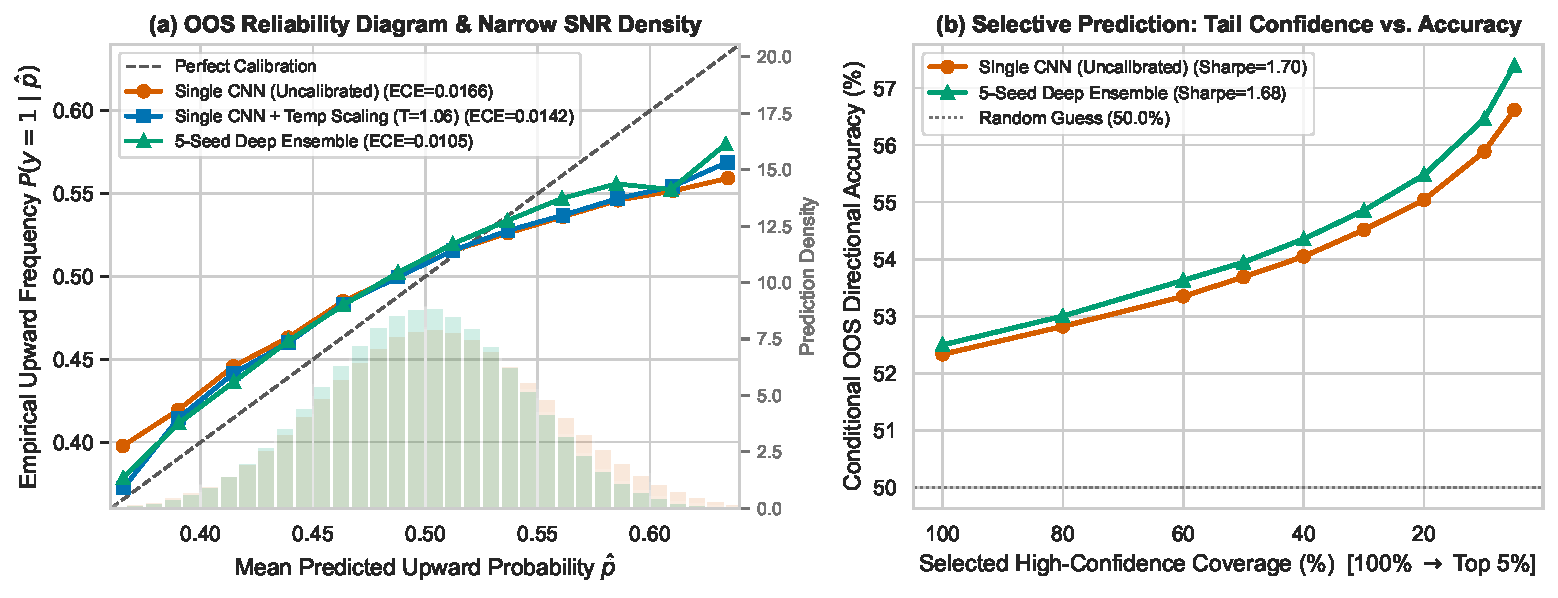
\includegraphics[width=\textwidth]{../outputs/figures/fig3_sq3_calibration.pdf}
  \vspace{-12pt}
  \caption{\textbf{RQ3 Probability Calibration and Selective Prediction (2000--2019 OOS, $N=1,491,887$).} \textbf{(a)} Zoomed reliability diagram over the active low-SNR probability support $[0.36, 0.64]$ overlaid with empirical prediction density histograms. \textbf{(b)} Conditional directional accuracy across top-$k\%$ confidence slices ranked by $|\hat{p} - 0.5|$.}
  \label{fig:sq3}
  \vspace{-6pt}
\end{figure}

\subsection{Empirical Findings: Variance Reduction Outperforms Post-Hoc Rescaling}
Table~\ref{tab:sq3} and Figure~\ref{fig:sq3} yield three key statistical insights:

\textbf{1. Mild Single-Model Overconfidence and Narrow SNR Support.} Unlike image classifiers on CIFAR/ImageNet whose outputs concentrate near $0$ and $1$, the background density in Figure~\ref{fig:sq3}(a) reveals that $>99\%$ of OOS financial chart predictions lie within the narrow interval $[0.36, 0.64]$. Even within this narrow band, a single CNN exhibits mild overconfidence: its reliability curve has a slope below unity (predicting $\hat{p} = 0.60$ corresponds to an empirical upward frequency of only $\approx 0.55$). Validation temperature scaling confirms this diagnosis by estimating $T = 1.064 > 1$, shrinking extreme logits toward zero and reducing single-model OOS ECE by $14.5\%$ ($0.0166 \to 0.0142$) and CE loss from $0.6924$ to $0.6921$.

\textbf{2. Deep Ensembling Achieves Superior Calibration without Distribution-Shift Fragility.} Averaging five seeds cuts OOS ECE by \textbf{51.2\%} relative to the single-seed average ($0.0215 \to 0.0105$, and $36.7\%$ below \texttt{seed=42}), aligning the green reliability curve closely with the $45^\circ$ diagonal in Figure~\ref{fig:sq3}(a) while simultaneously lifting AUC from $0.5322$ to $0.5355$. Notably, applying post-hoc temperature scaling \emph{on top of} the ensemble yields an in-sample validation temperature of $T_{\text{ens}} = 0.878 < 1$ (sharpening the averaged probabilities to match higher 1993--1999 in-sample predictability, where validation accuracy reaches $\approx 54.1\%$), which actually \emph{worsens} 2000--2019 OOS ECE from $0.0105$ to $0.0155$. This finding highlights a classic non-stationary pitfall: parametric post-hoc calibration fitted on a higher-SNR historical regime can over-sharpen probabilities when deployed into a more efficient modern market, whereas non-parametric ensemble averaging remains naturally well-calibrated.

\textbf{3. Selective Prediction Reconciles Modest Overall Accuracy with High Sharpe Ratios.} A recurring puzzle in financial ML is how a classifier with $52.50\%$ full-sample accuracy generates an annualized Sharpe ratio near $1.7$. Figure~\ref{fig:sq3}(b) resolves this via \emph{selective prediction}: ranking observations by confidence margin $|\hat{p} - 0.5|$ and progressively abstaining on ambiguous interior stocks causes OOS accuracy to rise strictly monotonically. For the 5-Seed Ensemble, directional accuracy climbs from $52.50\%$ at $100\%$ coverage to $53.95\%$ at $50\%$ coverage, \textbf{55.48\%} at $20\%$ coverage (precisely the combined universe of the top-$10\%$ long and bottom-$10\%$ short deciles, $|\hat{p}-0.5| \ge 0.057$), \textbf{56.46\%} at $10\%$ coverage, and \textbf{57.40\%} (AUC $0.5770$) in the top-$5\%$ confidence tail ($74,594$ trades, $+0.78$ percentage points above the single CNN at the same coverage). Cross-sectional decile portfolios act as an implicit selective-prediction filter that harvests the high-SNR tails while discarding the noisy near-$0.50$ bulk.

% =============================================================================
% SECTION 6: RQ4 SLOT (Member D)
% =============================================================================
\section{RQ4: Temporal Concept Drift and Grad-CAM Visual Attribution}
\teammatebox{Member D --- Section 6 ($\approx 1.4$ pages, includes Table 3 + Figure 4)}{%
  \textbf{Planned Content:} (1) Year-by-year rolling OOS trajectory from 2000 to 2019 across dot-com decimalization, the 2008 financial crisis, and 2010s algorithmic trading; head-to-head comparison of \texttt{Model\_1990s} (1993--1999) vs.\ \texttt{Model\_Modern} (2006--2012) on the common 2013--2019 test panel ($N=472,357$). (2) Case-study and Top-1000 population-averaged Grad-CAM attribution maps on Block 3 of \texttt{CNN20D}.%
}

% =============================================================================
% SECTION 7: CONCLUSION, CONTRIBUTIONS & AI STATEMENT (Framework Ready)
% =============================================================================
\section{Conclusion, Team Contributions, and AI Usage Disclosure}

\subsection{Conclusion and Limitations}
By auditing chart-based return CNNs across architecture, supervision, calibration, and temporal deployment, we show that Visual Alpha is statistically real and persistent over two decades of U.S.\ equity data, yet governed by tight bias--variance and low-SNR constraints. Deep ensembling substantially improves both ranking quality and probability calibration without post-hoc rescaling fragility, while selective tail prediction bridges the gap between $52.5\%$ overall classification accuracy and $1.7+$ portfolio Sharpe ratios. In the single-seed supervision comparison, keeping near-zero training returns preserved ranking quality, and smoothing all binary targets modestly improved calibration. \textit{[Add RQ1 and RQ4 findings at integration.]} Key limitations include equal-weighted portfolio construction without bid-ask transaction cost deductions and monthly snapshot rebalancing; incorporating turnover-penalized portfolio optimization represents a promising direction for future work.

\subsection*{Team Member Contributions}
\begin{itemize}[leftmargin=1.5em,itemsep=1pt,topsep=2pt]
  \item \textbf{Hanchong Qiu (Team Leader, Member A):} Designed overall four-stage research architecture and engineering contracts; implemented the shared \texttt{visual\_alpha} memory-mapped package and unified evaluator; executed 5-seed Baseline CNN replication and RQ3 calibration/selective-prediction experiments; authored Sections 1, 2, and 5.
  \item \textbf{[Member B Name] (Member B):} Implemented RQ1 cross-family inductive bias models (PCA+LR, LightGBM, 1D-CNN, ResNet) and spatial masking ablations; generated Table 2 and Figure 1; authored Section 3.
  \item \textbf{Dongqing Zhao (Member C):} Implemented RQ2 margin-filtering ($\tau$ and $t$-stat thresholds), label smoothing, and multi-horizon (5d/20d/60d) experiments; compared matched horizons and paired monthly returns, produced Figure~\ref{fig:sq2}, and wrote Section~\ref{sec:sq2}.
  \item \textbf{[Member D Name] (Member D):} Implemented RQ4 modern retraining concept-drift experiments and individual/aggregate Grad-CAM visual attribution; generated Table 3 and Figure 4; authored Abstract, Section 6, Section 7, and coordinated final manuscript \& presentation integration.
\end{itemize}

\subsection*{Statement on AI and Large Language Model Usage}
In accordance with MSDM 5054 course policy, we disclose the use of AI assistance (GitHub Copilot Agent in VS Code) during this project: (1) assisting with Python environment configuration (\texttt{uv}), memory-mapped \texttt{np.memmap} data-loader scaffolding, and PyTorch/Matplotlib boilerplate code; (2) diagnosing platform-specific runtime issues on Apple Silicon (\texttt{mps} backend and OpenMP library ordering); and (3) polishing academic English phrasing and \LaTeX{} table formatting. For RQ2, OpenCode assisted with experiment implementation and execution. OpenAI Codex assisted with the evaluation plan, prediction checks, statistical interpretation, figure, manuscript, and presentation. Section~\ref{sec:sq2} reports metrics computed from saved model predictions. \textit{[Update with teammates' AI log entries prior to submission.]}

\begin{thebibliography}{9}
\small
\setlength{\itemsep}{1.5pt}

\bibitem{jiang2023reimagining}
Jingwen Jiang, Bryan Kelly, and Dacheng Xiu.
\newblock (Re-)Imag(in)ing price trends.
\newblock \emph{The Journal of Finance}, 78(6):3193--3249, 2023.

\bibitem{gu2020empirical}
Shihao Gu, Bryan Kelly, and Dacheng Xiu.
\newblock Empirical asset pricing via machine learning.
\newblock \emph{The Review of Financial Studies}, 33(5):2223--2273, 2020.

\bibitem{guo2017calibration}
Chuan Guo, Geoff Pleiss, Yu Sun, and Kilian Q.\ Weinberger.
\newblock On calibration of modern neural networks.
\newblock In \emph{Proceedings of the 34th International Conference on Machine Learning (ICML)}, pages 1321--1330, 2017.

\bibitem{lakshminarayanan2017simple}
Balaji Lakshminarayanan, Alexander Pritzel, and Charles Blundell.
\newblock Simple and scalable predictive uncertainty estimation using deep ensembles.
\newblock In \emph{Advances in Neural Information Processing Systems (NeurIPS)}, volume 30, 2017.

\bibitem{selvaraju2017gradcam}
Ramprasaath R.\ Selvaraju, Michael Cogswell, Abhishek Das, Ramakrishna Vedantam, Devi Parikh, and Dhruv Batra.
\newblock Grad-CAM: Visual explanations from deep networks via gradient-based localization.
\newblock In \emph{Proceedings of the IEEE International Conference on Computer Vision (ICCV)}, pages 618--626, 2017.

\bibitem{jegadeesh1993returns}
Narasimhan Jegadeesh and Sheridan Titman.
\newblock Returns to buying winners and selling losers: Implications for stock market efficiency.
\newblock \emph{The Journal of Finance}, 48(1):65--91, 1993.

\bibitem{lo2000foundations}
Andrew W.\ Lo, Harry Mamaysky, and Jiang Wang.
\newblock Foundations of technical analysis: Computational algorithms, statistical inference, and empirical implementation.
\newblock \emph{The Journal of Finance}, 55(4):1705--1765, 2000.

\end{thebibliography}

\end{document}
